\input{configuration}

\title{Lecture 34 --- DevOps: Configuration }

\author{Patrick Lam \& Jeff Zarnett \\ \small \texttt{patrick.lam@uwaterloo.ca} \texttt{jzarnett@uwaterloo.ca}}
\institute{Department of Electrical and Computer Engineering \\
  University of Waterloo}
\date{\today}


\begin{document}

\begin{frame}
  \titlepage

 \end{frame}



\begin{frame}
\frametitle{DevOps for P4P}

\large

So far, one-off computations:
you need to answer a question, so you write code to do that.

But many systems are long-running (``generally available'').\\
$\Rightarrow$ Operations.

\end{frame}



\begin{frame}
\frametitle{Keep it Rolling}

\Large
Cloud computing: often long-lived systems,\\
but we didn't talk about how.\\[1em]
Today: many companies fuse\\
development (writes the software) \\
and operations (tends the software).

\end{frame}



\begin{frame}
\frametitle{Disaster Girl Strikes Again}

\begin{center}
	\includegraphics[width=0.8\textwidth]{images/devops.jpg}
\end{center}

\end{frame}



\begin{frame}
\frametitle{Start Me Up}

\Large

Startups:\\[1em]
No money to pay for separate \\
developer and operations teams.\\[1em]
Not that many servers, \\
just a few demo systems, test systems, etc\ldots\\
but it spirals out from there. \\[1em]
You're not really going to ask Sales to manage these servers, are you? \\
So, there's DevOps. 


\end{frame}



\begin{frame}
\frametitle{DevOps---Good Plan?}

\large

Is DevOps a good idea? \\
Can be used for both good and evil. \\[1em]
Good:
\begin{itemize}
\item developers involved across the software lifecycle.\\
(can learn a lot doing ops\ldots )
\item developers motivated to use correct tools \& document processes.
\end{itemize}


\end{frame}



\begin{frame}
\frametitle{Continuous Integration}

Each change or related group of changes is evaluated:

\begin{itemize}
	\item Pull from version Control
	\item Build
	\item Test
	\item Report results
\end{itemize}

Social convention to not break the build! Slack/Teams/etc. notifications.

\end{frame}


\begin{frame}
\frametitle{Configuration as Code}

\large

Systems have long come with \\
complicated (``flexible'') configuration options.


Sendmail is particularly notorious, but apache and nginx aren't super
easy to configure either.

First principle: treat \emph{configuration as code}.


\end{frame}



\begin{frame}
\frametitle{Configuration as Code}

\large

\begin{itemize}
\item use version control on your configuration.
\item implement code reviews on changes to the configuration.
\item test your configurations.
\item aim for a suite of modular services that integrate together smoothly.
\item refactor configuration files.
\item use continuous builds.
\end{itemize}


\end{frame}



\begin{frame}
\frametitle{Autoconfig}

\large

Excellent idea: tools for configuration. \\[1em]

Not enough to write text \\
\qquad ``How to Install AwesomeApp'' \\[1em]

e.g. use Terraform---\\
build, installation, and update automatic \& simple.\\[1em]

 Complicated means mistakes\ldots people forget steps. They are human. 
 
 
\end{frame}


\begin{frame}
\frametitle{Terraform}

\begin{center}
	\includegraphics[width=0.5\textwidth]{images/terraform.png}
\end{center}

Its whole purpose is to manage your config as codes
situation where you want to run your code using a cloud provider (e.g., AWS), 

\end{frame}


\begin{frame}
\frametitle{Planning is Essential}

Terraform has a ``plan'' operation: can verify the change it's about to make. 

Verify that we aren't about to give all our money to Jeff Bezos but also that a small change is actually small.

If you are happy with the change, apply it -- but things can change between plan and apply!

\end{frame}


\begin{frame}
\frametitle{Destructive Changes}

You can accidentally tell it you want to destroy all Github groups and people DM you thinking that this means they got fired.

\begin{center}
	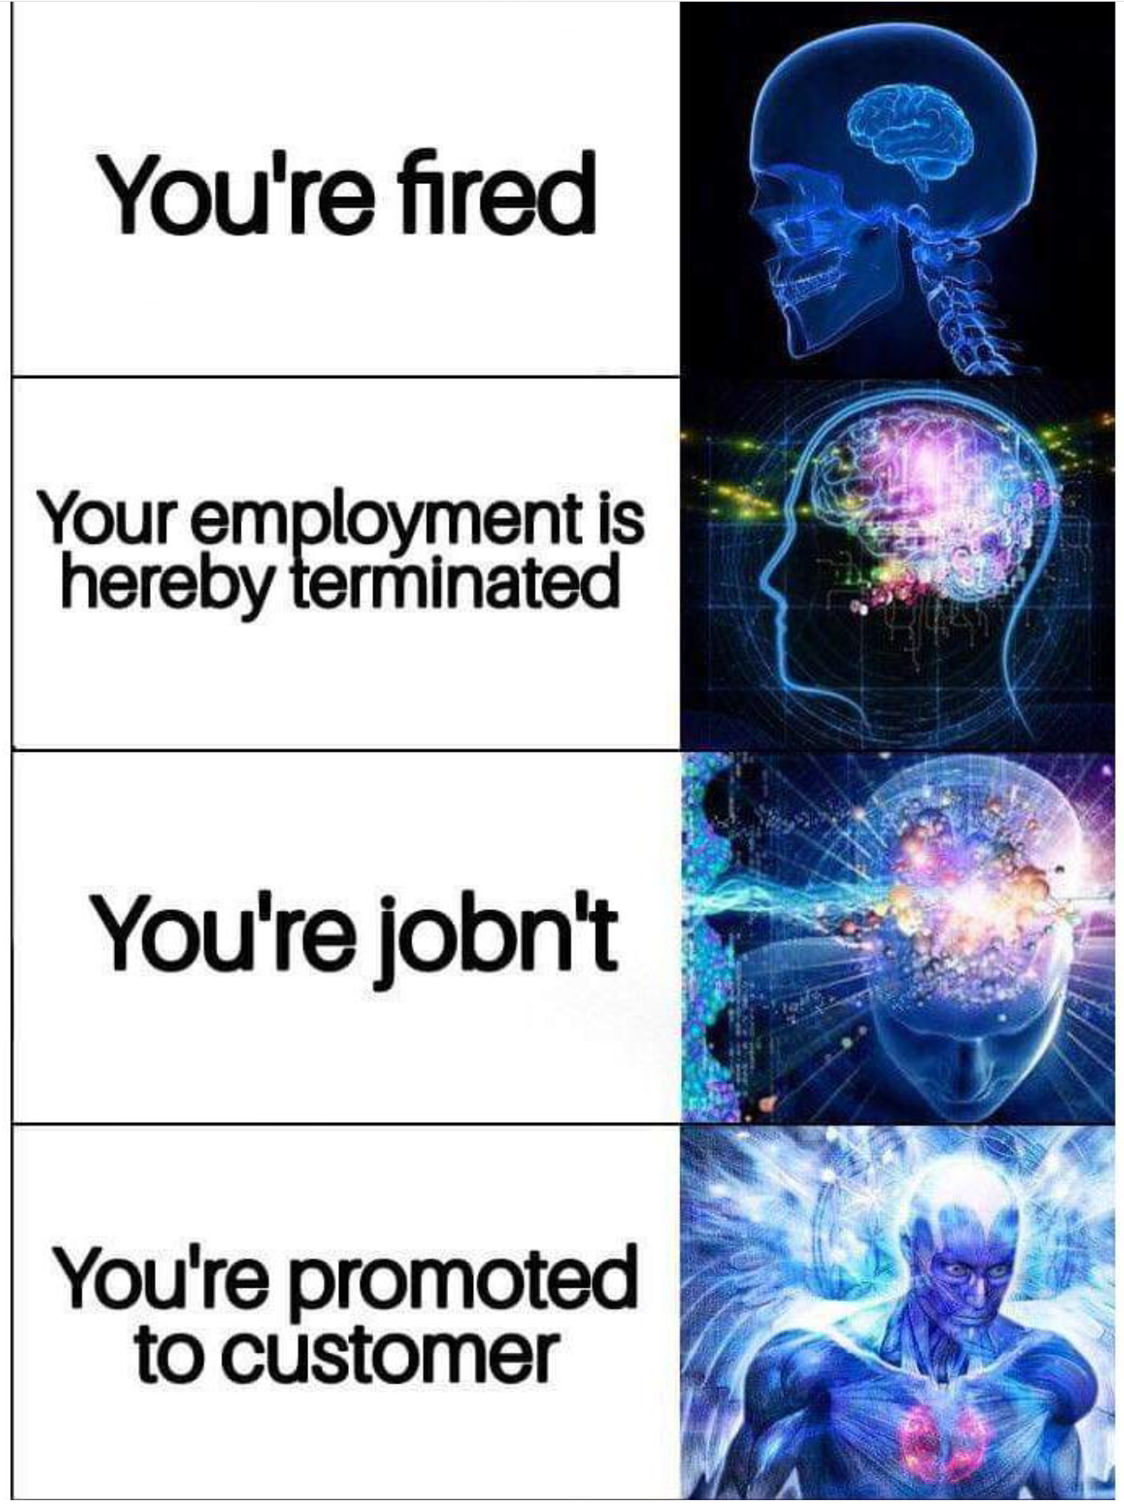
\includegraphics[width=0.4\textwidth]{images/fired.jpg}
\end{center}

\end{frame}

\begin{frame}
\frametitle{Common Infrastructure}

\large

Use APIs to access your infrastructure. Examples:

\begin{itemize}
\item storage
\item naming and discovery
\item monitoring
\end{itemize}

Avoid one-offs---use open-source tools when applicable.\\
But build your own tools if needed.


\end{frame}

\begin{frame}
\frametitle{Oh, Think Twice...}

Is this what we are best at?

Think extra carefully if you plan to do roll your own anything that is security or encryption related.

Remember that platforms like AWS are constantly launching new tools.

\end{frame}

\begin{frame}
\frametitle{Naming}

\Large

Naming is one of the hard problems in computing. 

There are only two hard things in computers:
\begin{enumerate}
\item cache invalidation,
\item naming things, and
\item off by one errors.
\end{enumerate}

\end{frame}



\begin{frame}
\frametitle{Naming Suggestions}

\large

\begin{itemize}
\item use canonical one-word names for servers;
\item but, use aliases to specify functions: geography/environment/purpose/serial
\end{itemize}


There's also the Java package approach of infinite dots: live.application.customer.webdomain.com

Pick something and be consistent.

\end{frame}


\begin{frame}
\frametitle{Billing or Potato?}

Debates rage about names should be meaningful or fun.

If the service is called \texttt{billing} it may be helpful in determining what it does, more so than if it were called \texttt{potato}.

But when you say the word do you mean the service or the team?

What if we need a new billing service? \texttt{billing2}

\end{frame}


\begin{frame}
\frametitle{Descriptive Names aren't Magic}

I've seen examples where the teams are called (anonymized a bit) ``X infrastructure'' and ``X operations''.

I'd estimate that 35\% of queries to each team result in a reply that says that the question should go to the other team. 

It gets worse when a team is responsible for a common or shared component (e.g., library). 

\end{frame}


\begin{frame}
\frametitle{Naming Solutions}

Real solution is like service discovery: tool with directory info.

Something like Opslevel exists; use it!

And don't forget that fun has a morale impact. 

\end{frame}

\begin{frame}
\frametitle{Servers as Cattle, not Pets}

\large

Servers means servers, or virtual machines, or containers.\\[1em]

At scale (smaller than you think):\\
use mass tools for dealing with servers, \\
rather than doing tasks manually. \\[1em]

At least: cloud-like server initialization without manual intervention;\\
must be able to spin up a server programmatically.


\end{frame}



\begin{frame}
\frametitle{Another Example}

\begin{center}
	\includegraphics[width=0.5\textwidth]{images/Kubernetes.jpg}
\end{center}

This is used to automate deploying and scaling of applications.

\end{frame}

\begin{frame}
\frametitle{Canarying}

\begin{center}
	\includegraphics[width=0.9\textwidth]{images/blackcanary.jpg}
\end{center}

\end{frame}



\begin{frame}
\frametitle{Canarying}

\large

Deploy new code incrementally in production, \\
also known as ``test in prod'':


\begin{itemize}
\item stage for deployment;
\item remove canary servers from service;
\item upgrade canary servers;
\item run automatic tests on upgraded canaries;
\item reintroduce canary servers into service;
\item see how it goes!
\end{itemize}

Of course: implement your system with rollback.


\end{frame}







\begin{frame}
\frametitle{Containerize Me, Captain}

\begin{center}
	\includegraphics[width=0.7\textwidth]{images/container.jpeg}
\end{center}

\end{frame}


\begin{frame}
\frametitle{How Did We Get Here?}

\begin{itemize}
	\item Manual install
	\item Package Manager (RPM/JAR/DLL Hell)
	\item Virtual Machines
	\item Containerization
\end{itemize}


\end{frame}


\begin{frame}
\frametitle{Containers}

See this diagram from NetApp:

\begin{center}
	\includegraphics[width=0.7\textwidth]{images/cvm.png}
\end{center}


\end{frame}





\end{document}

